\documentclass[10pt]{beamer}

\usepackage[utf8]{inputenc}
\usepackage{tcolorbox}
\usepackage{tikz}
\usepackage{tikz-3dplot}
\usetikzlibrary{intersections,calc,,angles,quotes,through}
\usepackage{amsmath}
\usepackage{graphicx}
\usepackage{cases}
\def \heart {\textcolor{blue}{$\heartsuit$} }
\def \C {\mathcal{C}}
\def \orthog {\underline{\perp}}
\def\arcos{\operatorname{arcos}}
\def \deg {^{\circ}}

\newcommand{\vect}[1] {
  \overrightarrow{#1}}

\tcbset{%
	basic/.style={colframe=black,
		      colback=white,
		      top= 0mm,
		      bottom = 2mm,
		      boxsep=0mm
		      }
}
\tikzset{
    invisible/.style={opacity=0},
    visible on/.style={alt={#1{}{invisible}}},
    alt/.code args={<#1>#2#3}{%
      \alt<#1>{\pgfkeysalso{#2}}{\pgfkeysalso{#3}} % \pgfkeysalso doesn't change the path
    },
  }

    
\begin{document}  
    \beamertemplatenavigationsymbolsempty
    \setlength{\abovedisplayskip}{0pt}
    \setlength{\belowdisplayskip}{0pt}
    \frame{
	  
	  \frametitle{Exemple de démonstration.}
	  %\renewcommand{\theenumi}{\alph{enumi})}
	  On considère un cercle $\C$ de centre $O$ et de rayon $r$, et un point $P$. Une droite $d$ issue
	  de $P$ coupe le cercle $\C$ en deux points $A$ et $B$. \\
	  On appelle la puissance du point $P$ par rapport au cercle $\C$ le produit scalaire $$\vect{PA}\cdot\vect{PB}$$
	  Propriété : La puissance de $P$ ne dépend pas l'inclinaison de $d$.
	  \vfill
	  
	  \pause
	  % hypothèses et thèse
	  \begin{tcolorbox}[basic] 
	      \begin{columns}[t]
		 
		 \column{.5\textwidth}\centering
		      
		      \underline{Hypothèses} 
		      \begin{itemize}
		      \item $AB$ corde de $\C$.
		      \end{itemize}

		  
		  \column{.5\textwidth}\centering
		      
		      \underline{Thèse} \\
		      \smallskip
		      $\vect{PA}\cdot\vect{PB}$ indépendant de $A,B$.
		
	      \end{columns}
	  \end{tcolorbox} \bigskip
	   {\small Référence : BELLIGOI T.,BASTIN F., 2011. \textit{Géométrie et géométrie analytique.} Disponible sur le site de la faculté, 169p.}
    } 
     
    

    \frame{ 
	  % résolution ex1
	  \begin{columns}[t]
		\column{.5\textwidth}\centering 
		

			\underline{Dessin}\\
			
				  \begin{figure}[h]
				  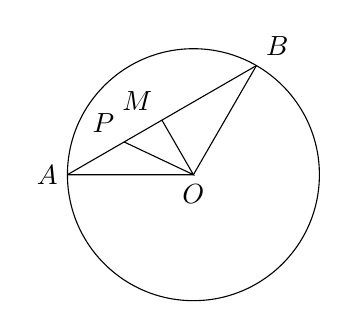
\begin{tikzpicture}[scale=0.8]
			          %projection ($(X)!(B')!(B)$)
			          %nommer chemin 'name path
			          %intersection \path [name intersections={of=d and gb,name=G}];
			          %animation  \draw[visible on=<1>] 
				  %           \draw[visible on=<{2,4}>]
				  %angle arc[radius = 6mm, start angle= 180, end angle= 225] node [below left,pos=0.3]{$\alpha$}
				  %angle \pic [draw,"$\alpha$", angle eccentricity=1.5] {angle = A'--A--B};
				  %perpendiculaire ($(A')!3cm!-90:(A)$)
				  %cercle par point \node [draw] at (A) [circle through=(B)] {};
				  
				  \coordinate[label=below:$O$] (O) at (0,0);
				  \coordinate[label=left:$A$] (A) at (-2,0);
				  \coordinate[label=above right:$B$] (B) at (60:2);
				  \coordinate[label=above left:$P$] (P) at ($(A)!0.3!(B)$);
				  \coordinate[label=above left:$M$] (M) at ($(A)!0.5!(B)$);
				  \draw (O) circle (2);
				  \draw (A) -- (B);
				  \draw (A) -- (O) -- (B);
				  \draw (P) -- (O) -- (M);
				  \end{tikzpicture}
				  \end{figure}
			
				  \begin{tcolorbox}[basic] 
				      
				    \smallskip
				    \underline{Hypothèses} 
				    \begin{enumerate}
				    \item $AB$ corde de $\C$. 
				    \end{enumerate}
							      
				    \underline{Thèse} \\
				    \smallskip
				    $\vect{PA}\cdot\vect{PB}$ indépendant de $A,B$.
				    \end{tcolorbox}
		
		
		\column{.5\textwidth}\centering
		
		\underline{Résolution}\\ \flushleft
		
		\begin{align*}
		 \vect{PA}\cdot\vect{PB} &=\ (\vect{PM}+\vect{MA})\cdot(\vect{PM}+\vect{MB}), \\[0.5em]				 
					 &=\ |\vect{PM}|^2 + \vect{PM}\cdot(\vect{MB} + \vect{MA}) - |\vect{MB}|^2, \\[0.5em]
					 &=\ |\vect{PM}|^2 - |\vect{MB}|^2, \\[0.5em]
					 &=\ |\vect{PO}|^2 - |\vect{OM}|^2 - (|\vect{OB}|^2 - |\vect{OM}|^2), \\[0.5em]
					 &=\ |\vect{PO}|^2 - |\vect{OB}|^2, \\[0.5em]
					 &=\ |PO|^2 - r^2. \\
		\end{align*}
		\hfill $\qed$
   
	   \end{columns}
    
    
    
    }
	  
  
\end{document}
